\chapter{Evaluating the performance of unmixing algorithms}

Our main goal is to evaluate performance of Nougad algorithm in both its momentum-based and ADAM variants against Ordinary Least Squares (OLS) and Weighted Ordinary Least Squares (WOLS) methods. 

We will also evaluate the performance for all the methods with the unmixing results clamped to zero --- negative abundance values in the unmixing result will be replaced with zeros.

\section{Generating artificial data sets}

To accurately and objectively measure the performance of various unmixing methods it is imperative to have a benchmark data set where ground truth is known. This is of course not possible when it comes to real world experiments since it is impossible to obtain ground truth abundances --- that is the reason are trying to find a better unmixing algorithm.

When generating such artificial data we should try to model the processes responsible for spectra emission and detection as accurately as possible while still keeping the model reasonably simple.

Note that we are generating Lymphocyte-like cells and their various sub-types only as this should be sufficient for testing purposes. However, if required it is easy to extend the phenotype table by additional cell types such as Monocytes.

The code responsible for generating the artificial data is available in supplementary materials as well as on Github\footnote{\url{https://github.com/mattejn/artificial_data_comp}}.

The general step-by-step process for generating artificial data is: 
\begin{enumerate}
\item{Obtain spectra for different fluorochromes.}
\item{Obtain phenotype characterizations for simulated cells.}
\item{Generate a fraction of dead cells for each phenotype}
\item{Simulate expression variability.}
\item{Simulate expression dependent noise.}
\item{Calculate cell emission spectra.}
\item{Simulate brightness-dependent noise.}
\end{enumerate}
  \subsection{Obtaining spectra for different fluorochromes} 
  Spectra can be either artificially generated and arbitrary or measured from single stain controls of a real experiment.  We decided to go with the latter to hopefully make the model more realistic however, this does not necessarily make the former approach less valid. The spectra was measured using the \texttt{R} application \texttt{PanelBuildeR} \footnote{\url{https://github.com/exaexa/panelbuilder}}.
  
  Either way the spectra form a standard unmixing matrix $M=D \cdot f$. Condition that states that there must be more individual detectors used for measurements than the number of distinct fluorochromes used in the experiment applies.
  
  Each fluorochrome is referred to by the name of the corresponding antibody from the reference real world experiment. 
  
  \subsection{Obtaining phenotype characterizations}
  In our approach phenotype matrix $P$ takes the form of $P=C_t*f$ giving probabilities of each fluorochrome $f$ (columns) for each cell type or sub-type $C_t$ (rows) --- each row in the matrix therefore represents an unique cell type.
  
  Furthermore, each row has a parent column that tells us what previously defined phenotype the current phenotype inherits abundances from. This allows us to only fill only the fluorochrome abundances that are different from the parent and leave the inherited blank, as in \cref{tab:packed_pheno}. 
  
  Relative cell counts for each phenotype are simply given by a vector $c$ of length $C_t$. Note that parent-child relationships are valid even for counts - this means that relative count for a child is a proportion of the parents relative count. 
  



  
\begin{table}
\small\sf
\label{tab:packed_pheno}
\begin{tabular}{lllcccccc}\toprule 
\multicolumn{2}{c}{Population}  &  \multirow{2}{3.5em}{Relative count} & \multicolumn{6}{c}{Antigens}\\ 
\cmidrule(l{.5em}r{.5em}){1-2}
\cmidrule(l{.5em}r{.5em}){4-9}
parent & current & {} & CD3 & CD56 & NKG2A  & CD4   & CD8   & AF\\
\midrule
-           & base    & 1             & 0   & 0    & 0      & 0     & 0     & 0  \\
base        & AF      & 0.95          &     &      &        &       &       & 1  \\
AF          & T       & 0.5           & 1   & 0    & 0.0052 & 0.738 & 0.224 &    \\
AF          & NK      & 0.2           & 0   & 1    & 1      & 0     & 0.14  &    \\
AF          & NK T    & 0.1           & 1   & 1    & 0.04   & 0.162 & 0.752 &    \\
T           & CD4     & 0.5           &     &      & 0      & 1     & 0     &    \\
CD4         & Thelper & 0.8           &     &      &        &       &       &   \\
\bottomrule
\end{tabular}
\caption{Example of a packed phenotype table.}
\end{table}


  This tree-like structure is then unpacked using a recursive function (available in the supplement) leaving us with a matrix that defines expression probability of each of the antibody targets for each cell type and their relative count in the resulting data set. $c$ is then normalized to one to give proportions of different phenotypes and multiplied by the desired number of cells for the entire data set giving us the extended probability matrix $Pex$.
  
  A partial example of an unpacked phenotype table with normalized relative counts is available in \cref{tab:unpacked_pheno}.
  
  When created $Pex$ is copied into $PexD$ which will be used to generate dead variations of the simulated cells. Finally $c$ is multiplied by $0.825$ scalar for $Pex$ and $0.175$ scalar for $PexD$ (creating $cd$) respectively - this represents the desired ratio of live ($82.5\%$) and dead ($17.5\%$) cells in the resulting data. This ratio is mostly arbitrary --- we simply wanted our data set to contain some number of dead cells without going overboard. Dead cell ratio can be changed using the appropriate parameter in the generator function or even disabled (set to 0).
  
  Absolute counts are rounded to the nearest integer.
  
\begin{table}\small\sf\
\label{tab:unpacked_pheno}
\begin{tabular}{lllcccccc}\toprule 
\multicolumn{2}{c}{Population}  &  \multirow{2}{3.5em}{Relative count} & \multicolumn{6}{c}{Antigens}\\ 
\cmidrule(l{.5em}r{.5em}){1-2}
\cmidrule(l{.5em}r{.5em}){4-9}
parent & current & {} & CD3 & CD56 & NKG2A  & CD4   & CD8   & AF\\
\midrule
AF          & NK       & 0.19     & 0   & 1    & 1     & 0     & 0.14  & 1  \\
AF          & NK T     & 0.095    & 1   & 1    & 0.04  & 0.162 & 0.752 & 1  \\
Thelper     & resting  & 0.1254   & 1   & 0    & 0     & 1     & 0     & 1  \\
Thelper     & effector & 0.0646   & 1   & 0    & 0     & 1     & 0     & 1  \\
Treg        & resting  & 0.03135  & 1   & 0    & 0     & 1     & 0     & 1  \\
Treg        & effector & 0.01615  & 1   & 0    & 0     & 1     & 0     & 1  \\
CD8         & naive    & 0.095    & 1   & 0    & 0     & 0     & 1     & 1  \\
\bottomrule
\end{tabular}
\caption{Partial example of a probability matrix from unpacked phenotypes.}
\end{table}
  
  \begin{algorithm}
  \caption{Extended probability matrix calculation}
  \label{alg:exprob}
  \begin{algorithmic}
  \State $cd \gets c$
  \State $Pex = []$
  \State $PexD = []$
  \State $a = 0$
  \State $b = 0$
  \For {$ i=1,..,N$}
  \State $c_i = c_i\div \sum{c}$
  \State $c_i = \lceil c_i \cdot m \cdot 0.825 \rfloor$
  \State $cd_i = \lceil c_i \cdot m \cdot 0.175 \rfloor$
  \For{$ k=a,..,(a+c_i$)}
  \State $Pex_{k*} = P_{i*}$
  \EndFor 
  \For{$ k=b,..,(b+cd_i$)}
  \State $PexD_{k*} = P_{i*}$
  \EndFor 
  \State $a = a+c_i$
  \State $b = b+cd_i$
  \EndFor 
  \end{algorithmic}
  \end{algorithm}
  
  \Cref{alg:exprob} is responsible for extended probability matrix calculation where $N$ corresponds to length of $c$ and $m$ to desired number of cells. $Pex$ is therefore given by repeating each row from $P$ times $c_i$ - the appropriate element of $c$. Analogically for $PexD$ and $cd_i/cd$. 
  
  A small example of an extended probability matrix can be found in: \cref{tab:ex_prob}
  

\begin{table}[]\small\sf
\label{tab:ex_prob}
\begin{tabular}{lcccccc} \toprule 
\multirow{2}{*}{Population}  & \multicolumn{6}{c}{Antigens}\\ 
\cmidrule(l{.5em}r{.5em}){2-7}
{} & CD3 & CD56 & NKG2A  & CD4   & CD8   & AF\\
\midrule
AFNK.14          & 0   & 1    & 1     & 0     & 0.14  & 1  \\
AFNK.15          & 0   & 1    & 1     & 0     & 0.14  & 1  \\
AFNK T           & 1   & 1    & 0.04  & 0.162 & 0.752 & 1  \\
AFNK T.1         & 1   & 1    & 0.04  & 0.162 & 0.752 & 1  \\
T helper resting   & 1   & 0    & 0     & 1     & 0     & 1  \\
T helper resting.1 & 1   & 0    & 0     & 1     & 0     & 1  \\
T helper effector  & 1   & 0    & 0     & 1     & 0     & 1 \\
 \bottomrule
\end{tabular}
\caption{Partial example of an extended probability matrix.}
\end{table}
  
  Relative counts and even phenotypes could be randomly generated however, we decided to use a matrix kindly provided by the thesis advisor representing the typical phenotypes for human Lymphocytes and their ratios in a real experiment as this should again lead to a more realistic model.
  
  \subsection{Simulating dead cells}
  In a real world experiment it is very likely that a significant fraction of measured cells ends up somehow damaged or dead as a result of chemical stress, apoptosis, and other causes.
  
  To simulate this fact we have created $PexD$ matrix in the previous step. Expression probabilities in $PexD$ are row-wise (per cell) multiplied by $sd$ - a vector of scalars randomly sampled from 0.3--0.6 range with appropriate length. This vector represents attenuated expression in the damaged cells. 
  
  Furthermore, a column vector $LDd$ is aded to both $Pex$ and $PexD$ representing expression probabilities for `LIVE/DEAD blue' dye. This stain binds to free amines found in cells with a damaged membrane. Probability vector for these amines in $PexD$ is semi-randomly set in 0.6--1 range. 
  
  The semi-randomness stems from the fact that each element of $LDd$ - $LDd_i$ is actually calculated by randomly sampling from 0.3--0.5 range and then adding $1-sd_i$ where $sd_i$ is the appropriate element $sd$. Finally, since the maximum possible value for this formula is actually 1.1 any element $LDd_i>1$ is set to one. 
  
  This results in the 0.6--1 range that is somewhat inversely correlated with expression attenuation (the more attenuated the expression, the more damaged we expect the cell to be, which would lead to more free amines) and slightly biased to higher values.
  \begin{algorithm}
  \caption{Dead phenotypes probability matrix}\label{alg:deadprob}
  \begin{algorithmic}
  \State $nc = ncol(PexD)$
  \State $d = [N]$
  \For {$ i=1,..,N$}
  \State $d_i = RandSamp\langle0.3;0.6\rangle$
  \State $PexD_i = PexD_i \cdot d_i$
  \State $d_i = (1-d_i)+RandSamp\langle0.3;0.5\rangle$
  \If{$d_i>1$}
  \State $d_i=1$
  \EndIf
  \State $PexD_{i(nc+1)}=d_i$
  \State $Pex_{i(nc+1)}=0$
  \EndFor 
  \State $Pfull=\left[ \begin{array} {c} Pex \\ PexD\end{array}\right]$
  \end{algorithmic}
  \end{algorithm}
  Finally $Pex$ and $PexD$ are row-wise joined creating the full probability matrix $Pfull$. For pseudocode refer to \cref{alg:deadprob}.

  
  \subsection{Simulating expression variability}
  Spectral abundances and are generated from the probability matrix leveraging the fact that for real world experiments the positive populations are expected at around $10^4$ mark.
  
  Before generating the abundances we split our column vectors into strong and weak markers. Strong markers have higher abundance floor than weak markers. This means that we need to use different processes to generate abundance values for these subsets. 
  
  \begin{algorithm}
  \caption{Abundances from probabilities}\label{alg:abund}
  \begin{algorithmic}
  \State $u = 1.5$
  \State $s = {2,3,9,14,17,21}$
  \State $D = ncol(Pfull)$
  \For {$ i=1,..,N$}
  \For {$ k=1,..,D$}
  \If {$D \in s$}
  \State $Pfull_{ik}=10^{(4-u)+u\cdot SampBinom(Pfull_{ik})+SampNorm(mean=0,sd=0.2)}$
  \Else
  \State$Pfull_{ik}=10^{2+2\cdot SampBinom(Pfull_{ik})+SampNorm(mean=0,sd=0.2)}$
  \EndIf
  \EndFor 
  \EndFor 
  \State $Ex=Pfull$
  \end{algorithmic}
  \end{algorithm}
  
  To differentiate strong markers we raise the floor from $10^2$ that is set for weak markers to $10^{4-u}$ where $0<u<2$ in order to strengthen strong marker expression. We tested $u=1$ and $u=1.5$ sticking with the latter when generating data for the final evaluation. 
  
  In \cref{alg:abund} $N$ represents the number of rows in the probability matrix $Pfull$ and $D$ number of columns. Function \texttt{SampBinom} samples single value from binomial distribution with the provided probability (current element of $Pfull$) simulating probability-based expression in the current cell for the current conjugated antibody target. Function \texttt{SampNorm} samples a single value from normal distribution with the provided parameters - $\text{mean}=0$ and $\text{standard deviation}=0.2$ simulating natural variability for both "positive" and "zero" expression. 
  
  This process leaves us with Expression matrix $Ex$ with abundances ranging from $\sim 10^2$ to $\sim 10^4$. We consider $Ex$ ground truth - it represents real abundances without noise. The closer the unmixing algorithm can get to those values the better we consider its performance. 
  
  In order to simulate noise resulting from the total amount of conjugated antibodies bound to target proteins we add Gaussian noise with standard deviation proportional to the sum of expression in each cell. The 0.001 scaling factor is only an estimate and can be adjusted within reasonable bounds: \cref{alg:expr_noise}.
  
  \begin{algorithm}
  \caption{Expression based noise}\label{alg:expr_noise}
  \begin{algorithmic}
  \State $N = nrow(Ex)$
  \State $D = ncol(Ex)$
  \For {$ i=1,..,N$}
  \For {$ k=1,..,D$}
  \State $Ex_{ik}=Ex_{ik}+SampNorm(mean=0,sd=(\sum{Ex_{i*}})\cdot 0.001)$
  \EndFor 
  \EndFor 
  \end{algorithmic}
  \end{algorithm}
 
\subsection{Calculating cell emission spectra and noise}
Cell emission spectra are calculated as a matrix product of the abundance matrix $Ex$ and the mixing matrix $M$ giving us the emission matrix $Em$. Each row of $Em$ then represents the resulting emission spectrum of a given cell - gained by multiplying the individual fluorochrome spectra from $M$ by their respective abundances for the given cell and summing the results: \cref{eq:emission}.
\begin{equation}
 Em = Ex \times M 
 \label{eq:emission}
\end{equation}

We are adding zero mean Gaussian noise to each element of $Em$ with standard deviation given by L2 norm of the given cell vector which corresponds to the total energy of the given cell or its fluorescent power. Note that we are using L2 norm because it better corresponds to the signal energy in physics context than L1/Hamming norm used in the case of expression-dependent noise: \cref{alg:power_noise}.

\Cref{fig:2D_gen} illustrates how does adding luminance-based noise affect the data in 2 selected dimensions.

  \begin{algorithm}
  \caption{Fluorescent power based noise}
  \label{alg:power_noise}
  \begin{algorithmic}
  \State $N = nrow(Em)$
  \State $D = ncol(Em)$
  \For {$ i=1,..,N$}
  \For {$ k=1,..,D$}
  \State $Em_{ik}=Em_{ik}+SampNorm(mean=0,sd=(\sum{Em_{i*}^2})\cdot 0.0005)$
  \EndFor 
  \EndFor 
  \end{algorithmic}
  \end{algorithm}
  

 
\begin{figure}
 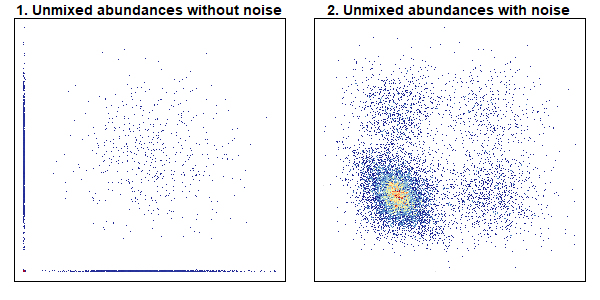
\includegraphics[width=1\linewidth]{img/2D_gen2.png}
 \caption{2D plot illustrating change caused by adding luminance-based noise.}
 \label{fig:2D_gen}
\end{figure}

\section{Nougad hyperparameter optimization}
 
\subsection{Multithread implementation of Nougad}
For the purpose of the hyperparameter optimization a significant speed boost for the Nougad algorithm was needed.

This is why we have modified the original code to allow parallel execution creating a multi-threaded fork of Nougad. Threading support is implemented directly in the $C$ function\footnote{\url{https://github.com/mattejn/nougad_mt}} which was not a trivial task for the author previously completely unfamiliar with $C$ programming language.

We also believe that this version will be helpful to others as vast majority of scientist has access to multi-threaded systems.

The speed improvement is very significant. For one million cells the unmixing time is reduced from $\sim$2 minutes to $\sim$6 seconds on 12 core/24 thread Ryzen 9 5900X CPU representing $\sim$20$\times$ speed increase (and purely by chance taking very similar amount of CPU time as the Moore-Penrose based calculation of OLS - which is of course single-threaded, on the very same CPU). 

Benchmark is available in supplemental materials as well as from Github\footnote{\url{https://github.com/mattejn/artificial_data_comp}} and as a part of the supplemental materials.

Linear performance increase is expected with increase in available CPU resources for single-CPU and most likely even multi-CPU systems.
 
\subsection{Available hyperparameters}
 
 Unlike OLS and WLS, Nougad is a tunable algorithm that gives us the option to influence its performance and behavior by changing its hyperparameters.
 
 Tunable parameters:
 \begin{enumerate}
    \item \emph{Spectra negative/positive weights - \param{snw}/\param{spw} }

    
    These parameters serve to weight the contribution of individual residuals when calculating the gradient, allowing us to set a bias towards/against positive/negative residuals. These scalars get converted to a weighting matrix. 

    \item \emph{Weights of non-negative learning factor - \param{nw}} 

    
    This gets converted to a vector of length $f$ and serves a bias against negative spectral abundances in the results. The higher this parameter is set the higher the cost for negative abundances becomes. It can be set as vector which could potentially be useful if we had a good reason to disproportionately "distrust" some of the spectra in a particular experiment.

    \item \emph{Starting points for gradient descent - \param{start}}

    
    Option that controls the starting points for abundance matrix. Setting this closer to a median abundance value for the unmixed data set could improve performance/reduce the number of iterations needed to reach a good result.

    \item \emph{Learning rate - \param{alpha}} 

    
    Scalar for the iterative update. Setting this too high can potentially lead to overflows/underflows and produce \texttt{NaNs}.
    
    \item \emph{Acceleration factor  - \param{accel}}  

    Scalar for the contribution of the previous update step to the current when the gradient direction (sign) remains unchanged. Setting this too high can lead to lead to overflows/underflows and produce \texttt{NaNs} while setting it too low will effectively disable the momentum based acceleration of this implementation.
     
    \item \emph{Number of iterations - \param{iters}}
    
    Number of iterations that will stop the algorithm when reached. 
\end{enumerate}
\begin{table}
\centering\footnotesize\sf
\begin{tabular}{ll}
\toprule
Parameter name & {Default value} \\
\midrule
\param{snw} & {1}  \\
\hline
\param{spw} & {1}\\
\hline
\param{nw} & {1}  \\
\hline
\param{start} & {0} \\
\hline
\param{alpha} & {0.01}  \\
\hline
\param{accel} & {1}  \\
\hline
\param{iters} & {250}\\
\bottomrule
\end{tabular}
\caption{Default hyperparameter values for Nougad}
\end{table}

\subsection{Bayesian hyperparameter optimization}
Exploring the hyperparameter space iteratively in its entirety is not feasible from a computational cost perspective. Of course, we could further reduce the explored ranges and increase step sizes or use a random search technique. Bayesian approach however seems like a more suitable option that could potentially lead to superior results.

Bayes theorem effectively allows us to calculate the conditional probability of event $A$ given $B$ when we know the prior probabilities for $A$ and $B$ and the conditional probability of $B$ given $A$: \cref{eq:bayes_base}. 

\begin{equation}
P(A|B)=\frac{P(B|A)P(A)}{P(B)}
\label{eq:bayes_base}
\end{equation}

In Bayesian optimization we leverage Bayes theorem coupled with several randomly selected pre-computed points from the hyperparameter space to probabilistically model the \emph{Surrogate function}. Surrogate function can be thought of as a function of the objective function (the function we are trying to minimize/maximize). Surrogate function takes the hyperparameter values and outputs the loss. 

After a set number of points in the hyperparameter space is precalculated, next point to sample is decided using the \emph{acquisition function}. 

Acquisition function usually takes into an account the exploration/exploitation trade-off - we want to select coordinates in the hyperparameter space that have the highest potential to maximally decrease loss, but at the same time we want to actually explore the space and avoid moving around one or multiple local minima. 

Once the next point is sampled the probabilistic model of the surrogate function is adjusted based on observed loss\cite{Bayes2016}. This process for a 1D problem - tuning a single hyperparameter, is well illustrated in \cref{fig:bayes_opt}.

\begin{figure}
  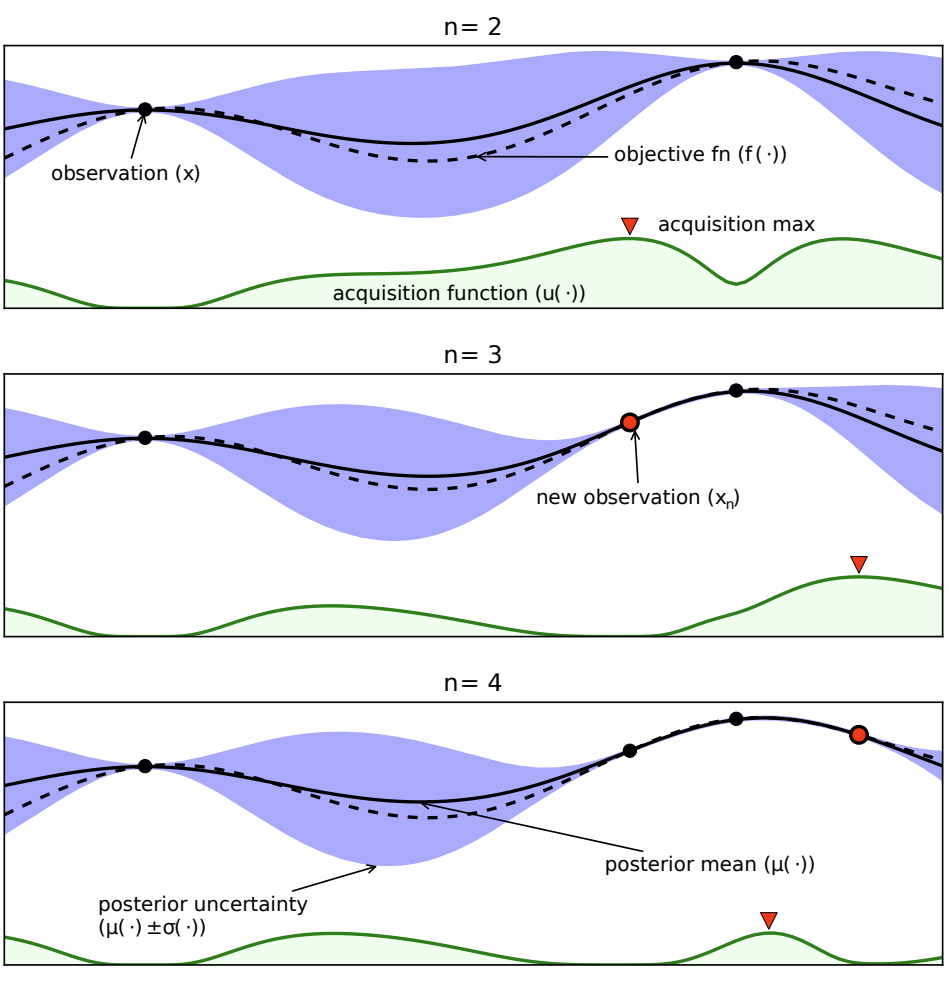
\includegraphics[width=120mm]{img/Bayes_opt.png}
  \caption{Overview of a 1-dimensional Bayesian optimization process. Image by~\citet{Bayes2016}.}
  \label{fig:bayes_opt}
\end{figure}

We used \texttt{mlrMBO} library\footnote{\url{https://mlrmbo.mlr-org.com/}} that implements Bayesian optimization and allows us to define our objective function we want to minimize. 

For the acquisition function we selected \texttt{ExpectedImprovement} mostly because it seems to perform well in most applications\cite{Bayes2016} and since we are leveraging multi-point evaluation in order to utilize multi-threading it will be its multipoint modification \texttt{q-EI}\cite{bayes_multipoint}.

In order to minimize overfitting concerns we generated four distinct data sets of 100 000 cells each, that differ in the characteristics of their strong markers - two have the same strong markers but with a different floor and two lack strong markers. Each data set also uses different random seed.

Loss is then calculated as average of mean squared errors of all three data sets after Nougad unmixing using the selected hyperparameters against their respective ground truths. We ran the model for 2000 iterations which required over 30 hours of computation time.

Note that deeper dive into Bayesian optimization, different acquisition functions and their properties is outside of the scope of this thesis. Everything needed for our application is well explained and illustrated in \cite{Bayes2016} which can also serve as a good starting point for any reader wishing to delve deeper. 

\subsection{Parameter ranges for tuning}
For \param{spw} and \param{spw} we decided to go with range of 1--300 since in preliminary testing with values up to 2000 there were no competitive results with either set over 300.

Similarly for \param{nw} we choose the ceiling of 2000 since in preliminary tests anything higher did not seem beneficial and would often lead to \texttt{NaN} results. Overall this is the parameter where we know for a fact that it must be set somewhat high to exploit the main advantage of Nougad - soft constraint for negative spectral abundances. 

For \param{start} we picked the range of 1--500 reasoning being that for our artificial data the median value after umixing and clamping to 0 using OLS, WLS or even less optimized Nougad tends to lie between 300--400 which is not far off the median value for ground truth. Setting this close to median of clamped unmixed result could work as a reasonable rule of thumb for real data as well.

We know that learning rate - \param{alpha} should not be set too high in order to avoid \texttt{NaN} results. This cutoff seems to be around 0.1 value from preliminary testing that was done in 0.001--1 range. Furthermore, values of over $0.02$ did not seem to provide competitive results overall. Range for more thorough testing was kept between 0.001--0.02 with increments of 0.001.

After some preliminary testing for \param{accel} with already established ranges for other parameters we settled on 0.001-1 with 0.001 increments. Values $> 1$ seem to produce \texttt{NaN} quite reliably when using higher values for \param{nw} (which is necessary to improve Nougad performance).

Overall there is varying degree of interplay between all parameters so their values cannot really be discussed in a vacuum (maybe with the exception of \param{start}).

Finally even though our chosen optimization strategy allows us to set continuous ranges for all the parameters we decided to not leverage this option. Mostly for simplicity, but also because there seems to be no argument as to why this option would lead to a significantly improved results. Ranges are therefore in integers with $\text{step size} = 1$ unless otherwise specified.

\subsection{Tuning outcome}
We managed to reduce mean squared error on testing data set almost two-fold when compared to manual tuning and almost four-fold when compared to default values of Nougad function (which behave indentically to OLS).

The script used for tuning (including the custom objective function and hyperparameter ranges) is available in the supplement.
 
\section{Unmixing quality metrics}
The main advantage of the simulated data is that we can objectively and easily measure the difference between the two $n \cdot m$ matrices --- the abundance matrix $U$ produced by currently evaluated unmixing algorithm and the ground truth abundance matrix $A$. Mean squared error (MSE) is perfectly suitable for this:
\[MSE=\frac{1}{nm}\sum_{i=1}^{n}\sum_{k=1}^{m}(A_{ik}-U_{ik})^2\]
In other words we are computing the mean of elementwise squared error between the two abundance matrices.

The reason we are using squared error is that emphasizes outliers and de-emphasizes small noise. Both of those things are desirable for us. We don't really mind if a cell is shifted by a fraction from its real coordinates, however big location shifts in our multidimensional space are problematic and can lead to some fundamentally incorrect conclusions. 

We will also be looking at per cell MSE, squared error distribution over the entire data set and in individual spectra and spectra pairs. Finally we leverage embedding and dimensional reduction using Self-Organazing Maps (SOM) implemented in R package EmbedSOM\cite{ESOMpap}. 

\subsection{Evaluation on real-world experimental data}

While simulated data should approximate the characteristics of real data, the truth is that no model is perfect.

As far as the author of this thesis knows no truly objective method for evaluating unmixing performance on data without known ground truth exists.

Despite this fact it is still useful to try to visualize and tentatively compare both real data from peripheral blood of a helthy patient and artificial.

\subsubsection{Comparison of artificial to real data}
Visualizations are done using UMAP assisted embedding into 2D using \texttt{EmbedSOM} library. 

First we take a look at the real and artificial data comparison. From \cref{fig:SOM_comp} we can see that clusters defined by the selected markers are present in both data sets. In artificial data there is significantly more fragmentation within these clusters which is caused by `sharply' defined phenotypes. This is not replicated in real data as some of the phenotypes are simply not present and there is even more noise for the ones that are.

\begin{figure}
  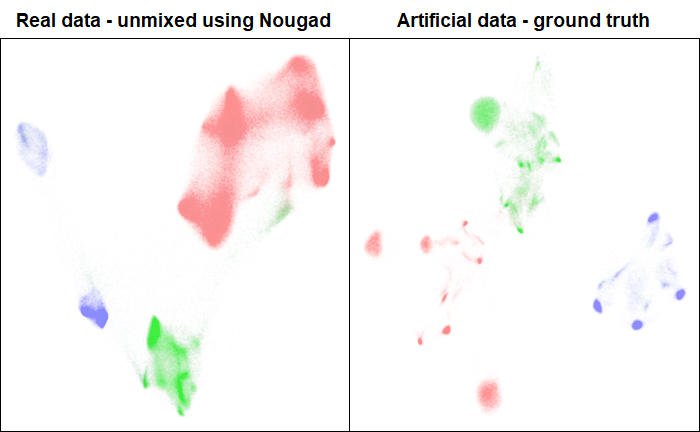
\includegraphics[width=1\linewidth]{img/SOM_comp_real_artv2.png}
  \caption{Comparison of real and artificial data --- colored by CD4 (red), CD8 (green) and CD16 (blue) markers.}
  \label{fig:SOM_comp}
\end{figure}

Ultimately there clearly are some fundamental differences between data sets however, broader structure in the artificial data seems similar enough to the real data for the purpose of unmixing method evaluation. 

